% Options for packages loaded elsewhere
\PassOptionsToPackage{unicode}{hyperref}
\PassOptionsToPackage{hyphens}{url}
\documentclass[
  11pt,
]{article}
\usepackage{xcolor}
\usepackage[margin=1in]{geometry}
\usepackage{amsmath,amssymb}
\usepackage{tikz}
\usetikzlibrary{positioning,arrows.meta}
\setcounter{secnumdepth}{-\maxdimen} % remove section numbering
\usepackage{iftex}
\ifPDFTeX
  \usepackage[T1]{fontenc}
  \usepackage[utf8]{inputenc}
  \usepackage{textcomp} % provide euro and other symbols
\else % if luatex or xetex
  \usepackage{unicode-math} % this also loads fontspec
  \defaultfontfeatures{Scale=MatchLowercase}
  \defaultfontfeatures[\rmfamily]{Ligatures=TeX,Scale=1}
\fi
\usepackage{lmodern}
\ifPDFTeX\else
  % xetex/luatex font selection
\fi
% Use upquote if available, for straight quotes in verbatim environments
\IfFileExists{upquote.sty}{\usepackage{upquote}}{}
\IfFileExists{microtype.sty}{% use microtype if available
  \usepackage[]{microtype}
  \UseMicrotypeSet[protrusion]{basicmath} % disable protrusion for tt fonts
}{}
\makeatletter
\@ifundefined{KOMAClassName}{% if non-KOMA class
  \IfFileExists{parskip.sty}{%
    \usepackage{parskip}
  }{% else
    \setlength{\parindent}{0pt}
    \setlength{\parskip}{6pt plus 2pt minus 1pt}}
}{% if KOMA class
  \KOMAoptions{parskip=half}}
\makeatother
\usepackage{longtable,booktabs,array}
\newcounter{none} % for unnumbered tables
\usepackage{calc} % for calculating minipage widths
% Correct order of tables after \paragraph or \subparagraph
\usepackage{etoolbox}
\makeatletter
\patchcmd\longtable{\par}{\if@noskipsec\mbox{}\fi\par}{}{}
\makeatother
% Allow footnotes in longtable head/foot
\IfFileExists{footnotehyper.sty}{\usepackage{footnotehyper}}{\usepackage{footnote}}
\makesavenoteenv{longtable}
\setlength{\emergencystretch}{3em} % prevent overfull lines
\providecommand{\tightlist}{%
  \setlength{\itemsep}{0pt}\setlength{\parskip}{0pt}}
\usepackage{bookmark}
\IfFileExists{xurl.sty}{\usepackage{xurl}}{} % add URL line breaks if available
\urlstyle{same}
\hypersetup{
  hidelinks,
  pdfcreator={LaTeX via pandoc}}

\author{}
\date{}

\begin{document}

\section{Epistemic Interdependence as a Design Principle for
AI-Generated Collaborative Mathematical Tasks: A Framework, Simulation
Method, and Pilot
Study}\label{epistemic-interdependence-as-a-design-principle-for-ai-generated-collaborative-mathematical-tasks-a-framework-simulation-method-and-pilot-study}

\textbf{Target}: International Journal of Computer-Supported
Collaborative Learning (IJCSCL), Springer\\
\textbf{Status}: Skeleton --- awaiting pilot v3 results\\
\textbf{Estimated length}: 8,000--10,000 words

\begin{center}\rule{0.5\linewidth}{0.5pt}\end{center}

\subsection{Abstract}\label{abstract}

Genuinely collaborative mathematical problem solving requires information splits that create \emph{epistemic interdependence} --- where neither participant can formulate a solvable approach without the other's contribution. Yet the structural conditions for such interdependence are difficult to design systematically, and simulating collaborative problem solving at scale introduces validity threats that have not been fully examined. This paper makes three contributions. First, we introduce the Collaborative Phase Profile (CPP) framework, a formal characterisation of collaborative problem solving as a binary vector over twelve PISA 2015 CPS cells (four problem-solving processes $\times$ three collaborative competencies), and the CPS Depth Index (CDI), a scalar measure of collaborative engagement depth in {[}0, 1{]}. Second, we report a behavioral solo-verification procedure that identifies 50\% of algorithmically generated information splits as behaviorally trivial --- solvable by a single agent without collaboration --- and establish that split quality varies substantially by structural pattern (SPLIT-F: 77\% genuinely interdependent; SPLIT-D: 33\%). Third, we present a scale study ($n = 321$ conversations: 36 behaviorally INTERDEPENDENT problems $\times$ 3 coordination protocol conditions $\times$ 3 replications) demonstrating that coordination protocol design produces large, reliable improvements in collaborative engagement. The plan-first student-simulation protocol (C10b) raises mean CDI from 0.747 ($\pm$0.261) to 0.967 ($\pm$0.086) relative to the student-simulation baseline (C7), with 80\% of C10b conversations activating all 12 PISA CPS cells versus 28\% under C7 (Cohen's $d = 1.16$, $p < 0.001$). Expert framing (CEXP) collapses CDI to 0.294 --- below the no-framing baseline (C2 = 0.322) --- confirming that agent framing is the primary determinant of collaborative emergence. A moderating analysis identifies probability and counting problems (SPLIT-F) as a context where the structured protocol improves CDI but reduces task accuracy, providing a principled basis for adaptive protocol selection. Implications for the design of AI-generated collaborative mathematical activities are discussed.

\begin{center}\rule{0.5\linewidth}{0.5pt}\end{center}

\subsection{1. Introduction}\label{introduction}

Collaborative problem solving (CPS) has emerged as a core
twenty-first-century competency (OECD, 2017), yet the design of tasks
that genuinely require collaboration --- rather than merely permitting
it --- remains an open challenge. In mathematics education, jigsaw-style
activities divide information across learners, but the division is
typically informational: once each learner shares their piece, a single
agent could complete the solution. This creates \emph{data splits}
rather than \emph{epistemic splits}, and the collaboration it elicits is
shallow: participants exchange data but do not jointly reason.

The advent of large language model (LLM) agents as proxies for learners
opens new methodological possibilities. LLM agents can be simulated at
scale, their interactions logged and scored automatically, and
controlled conditions can be tested before deployment with real
students. However, the design of these simulations conceals significant
choices: how to frame the collaborative context, what information to
provide each agent, and how to measure whether genuine collaborative
problem solving occurred.

This paper addresses three interrelated problems:

\begin{enumerate}
\def\labelenumi{\arabic{enumi}.}
\tightlist
\item
  \textbf{Theoretical}: What constitutes a genuinely epistemic split,
  and how can it be formally characterized?
\item
  \textbf{Methodological}: How can LLM agent simulation validly measure
  collaborative problem-solving depth?
\item
  \textbf{Empirical}: Which conditions most reliably produce deep
  collaboration, and under what circumstances does process quality
  predict correct outcomes?
\end{enumerate}

We contribute: - The CPP framework and CDI metric as formal tools for
characterizing CPS task design - A five-condition experimental design
with theoretical grounding for each condition - The Collaborative Yield
(CY) metric integrating process and outcome within a productive failure
framework - Evidence from a three-iteration pilot study of
methodological design decisions

\begin{center}\rule{0.5\linewidth}{0.5pt}\end{center}

\subsection{2. Theoretical Background}\label{theoretical-background}

\subsubsection{2.1 Collaborative Problem Solving: The PISA 2015
Framework}\label{collaborative-problem-solving-the-pisa-2015-framework}

The PISA 2015 assessment framework defines collaborative problem solving
as ``the capacity of an individual to engage effectively in a process
whereby two or more agents attempt to solve a problem by sharing the
understanding and effort required to come to a solution'' (OECD, 2017,
p.~134). The framework decomposes CPS into a 4 $\times$ 3 matrix: four
problem-solving processes (A: Exploring and Understanding; B:
Representing and Formulating; C: Planning and Executing; D: Monitoring
and Reflecting) crossed with three collaborative competencies (1:
Establishing and maintaining shared understanding; 2: Taking appropriate
action to solve the problem; 3: Establishing and maintaining team
organization).

This yields twelve cells (A1--D3) that operationalize where and how
collaboration occurs across the problem-solving trajectory. Prior
research has shown that jigsaw conditions elevate cells A1 (shared
exploration) and B1 (joint formulation) relative to solo conditions, but
frequently suppress C2 (mathematical execution action) --- suggesting
that conventional splits trade procedural performance for collaborative
engagement (see Results, this paper).

\subsubsection{2.2 Epistemic Splits vs.~Data
Splits}\label{epistemic-splits-vs.-data-splits}

\textbf{Data splits} partition known quantities across agents (Agent A
knows value x, Agent B knows value y; sharing x and y allows either
agent to complete the solution independently). \textbf{Epistemic splits}
partition \emph{reasoning roles}: Agent A must derive intermediate
values that Agent B needs to apply a different mathematical principle;
neither can formulate a solvable equation without the other's
contribution.

The distinction is operationalized through the \emph{epistemic fidelity
criterion}: a split has high epistemic fidelity if the point-biserial
correlation r\_pb(CDI, correctness) across conditions is positive and
significant for that problem. A data split produces r\_pb $\approx$ 0 because
CDI and correctness are statistically independent --- any agent can
stumble toward the answer without genuine collaboration.

\textbf{Design example} (math\_00121, sec $\theta$ + tan $\theta$ = 22/7): An
epistemic split assigns Agent 1 the given equation and the role of
deriving sin $\theta$ and cos $\theta$; Agent 2 receives the identity csc $\theta$ + cot $\theta$ =
(1 + cos $\theta$)/sin $\theta$ and the task of computing m + n from the reduced
fraction. Neither can proceed without the other's output. A data split
would give Agent 1 the equation and Agent 2 only ``find m + n'' ---
Agent 1 can derive the entire solution independently.

\subsubsection{2.3 Productive Failure and the Process-Outcome
Relationship}\label{productive-failure-and-the-process-outcome-relationship}

Kapur (2012) demonstrated that students who engage deeply with a problem
and fail produce better subsequent learning than students who succeed
with shallow engagement. This \emph{productive failure} finding reframes
the interpretation of high-process/incorrect-outcome pairs: they
represent maximal engagement within the ZPD, not educational failure.

For our framework, this implies that CDI and correctness cannot be
collapsed into a single metric without theoretical loss. The
Collaborative Yield (CY) metric (introduced in Section 3.6) preserves
this distinction while providing a practical composite for condition
ranking.

\subsubsection{2.4 The ICAP Framework}\label{the-icap-framework}

Chi and Wylie's (2014) ICAP framework predicts that interactive
engagement produces greater learning than constructive, active, or
passive engagement. In our context, interactive engagement corresponds
to cells requiring \emph{bidirectional knowledge construction} --- both
agents jointly building representations neither held alone. ICAP
predicts that conditions producing higher proportions of interactive
(rather than constructive or active) turns will show both higher CDI and
higher learning outcomes.

\subsubsection{2.5 Joint Accountability and the Convergence
Criterion}\label{joint-accountability-and-the-convergence-criterion}

Roschelle (1992) identified \emph{convergence} --- the process by which
collaborators negotiate a shared understanding and verify that both hold
the same representation --- as a defining feature of genuine joint
problem solving. Szewkis et al.~(2011) operationalize this as condition
4 (\emph{group reward orientation}): participants are accountable
collectively for the group's outcome. In our design, joint
accountability is implemented structurally: both agents must
independently state the same final answer. This is minimal (no
mid-conversation intervention), grounded in convergence theory, and
distinguishable from external facilitation --- which, when injected
during the problem-solving trajectory, risks measuring the facilitator's
effectiveness rather than the dyad's collaborative capacity.

\subsubsection{2.6 Task-Role Chain Design and the Epistemic Fidelity
Problem}\label{task-role-chain-design-and-the-epistemic-fidelity-problem}

A canonical approach to CPS task design assigns each participant private
information the other lacks, implying that ``you cannot solve this
alone'' (Dillenbourg, 1999). This creates a \emph{data split}. However,
with LLM agents --- which have unrestricted mathematical knowledge ---
knowledge restriction via prompt engineering is simulated, not genuine:
the agent ``knows'' the solution but is instructed to pretend otherwise.
More critically, the instruction \emph{pre-computes} the discovery of
information asymmetry, eliminating the exploration phase (PISA A1) in
which participants naturally discover what the other knows and needs
(Roschelle, 1992; Chi \& Wylie, 2014).

\emph{Task-role chain design} (introduced in this paper) resolves this
by assigning \emph{computational roles} rather than information
asymmetries. Each agent receives: (1) the inputs available to them, (2)
the computation to perform, (3) what to communicate to the partner, and
(4) what output they need from the partner to complete the chain. The
chain creates genuine functional interdependence --- neither agent can
produce the final answer without the other's intermediate result ---
while preserving Phase A by leaving the discovery of \emph{why} the
roles are interdependent to the collaborative conversation itself.

\begin{center}\rule{0.5\linewidth}{0.5pt}\end{center}

\subsection{3. Methodology}\label{methodology}

This paper reports two interrelated studies. The \textbf{pilot study} (§3.1--3.9) developed and validated the CPP framework and CIDI pipeline through a four-iteration design process on $n=4$ problems $\times$ 5 conditions. The \textbf{scale study} (§4) applied the validated framework to 36 behaviorally INTERDEPENDENT problems $\times$ 3 protocol conditions $\times$ 3 replications ($n=321$ conversations), providing the primary statistical evidence for the paper's claims. Sections 3.3--3.5 describe methodology shared by both studies; §3.4 introduces the full coordination protocol spectrum developed iteratively across the pilot phase.

\subsubsection{3.1 The CPP Framework and
CDI}\label{the-cpp-framework-and-cdi}

The Collaborative Phase Profile (CPP) is a binary vector \textbf{CPP $\in$
\{0,1\}\^{}12} over the twelve PISA CPS cells. For a given problem P and
split strategy S with n agents, CPP(P, S, n) indicates in which cells
collaboration is structurally necessary for problem resolution.

The CPS Depth Index is defined as:
\[CDI(P, S) = \frac{\sum_{i=1}^{12} cpp_i}{12} \in [0, 1]\]

CDI = 0 indicates no collaborative engagement is required or observed.
CDI = 1 indicates activation across all twelve cells. In practice, five
empirical profiles emerge: CPP-IC (\textless0.25), CPP-CG (0.25--0.42),
CPP-RP (0.42--0.58), CPP-DEEP (0.58--0.83), CPP-FULL (1.0).

\subsubsection{3.2 The CIDI Pipeline (Module
1--5)}\label{the-cidi-pipeline-module-15}

\begin{figure}[ht]
\centering
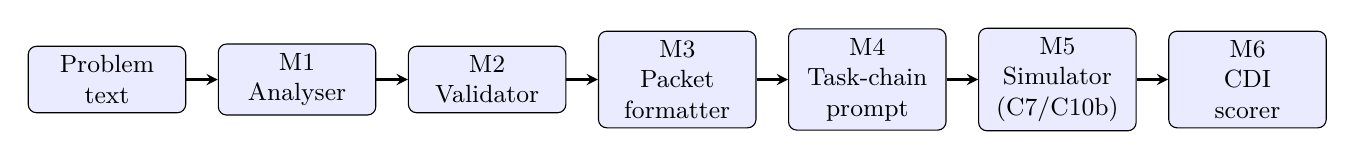
\begin{tikzpicture}[
    node distance=0.55cm and 0.4cm,
    box/.style={draw, rounded corners=3pt, fill=blue!8, minimum width=2.0cm, minimum height=0.7cm, font=\small, align=center},
    arrow/.style={->, >=stealth, thick},
]
\node[box] (prob) {Problem\\text};
\node[box, right=of prob] (m1) {M1\\Analyser};
\node[box, right=of m1] (m2) {M2\\Validator};
\node[box, right=of m2] (m3) {M3\\Packet\\formatter};
\node[box, right=of m3] (m4) {M4\\Task-chain\\prompt};
\node[box, right=of m4] (m5) {M5\\Simulator\\(C7/C10b)};
\node[box, right=of m5] (m6) {M6\\CDI\\scorer};

\draw[arrow] (prob) -- (m1);
\draw[arrow] (m1) -- (m2);
\draw[arrow] (m2) -- (m3);
\draw[arrow] (m3) -- (m4);
\draw[arrow] (m4) -- (m5);
\draw[arrow] (m5) -- (m6);
\end{tikzpicture}
\caption{The CIDI pipeline: six modules transform a problem text into a CDI-scored split. M5 uses protocol C10b for training data generation and C7 for held-out evaluation.}
\label{fig:cidi-pipeline}
\end{figure}

The Collaborative Interaction Design Infrastructure (CIDI) is a
six-module pipeline for generating CPP-targeted epistemic splits:

\begin{itemize}
\tightlist
\item
  \textbf{M1 --- Semantic Analysis} (LLM, Groq): Produces a problem
  anatomy including sub-problems, reasoning type, information
  bottlenecks, and natural split axes.
\item
  \textbf{M2 --- Feasibility DAG} (deterministic): Builds a directed
  acyclic graph of logical dependencies between sub-problems; computes
  DAG closure to derive reachable CPP profiles.
\item
  \textbf{M3 --- Constraint Derivation} (deterministic): Maps a target
  CPP profile to per-cell design instructions and entity assignment
  hints.
\item
  \textbf{M4 --- Linguistic Generation} (LLM): Translates the formal
  specification into natural-language information packets for each
  agent. Critically, M4 must generate \emph{epistemic} splits: the
  prompt forbids informational splits (neither agent should be able to
  formulate a solvable equation without the other).
\item
  \textbf{M5 --- CPP Discriminator Chain} (trained): 12 logistic
  regression classifiers in DAG order, each predicting one PISA cell's
  activation probability from TF-IDF features of simulated conversation
  turns. Trained on 140 annotated examples; mean Hamming error 1.11/12
  on validation set.
\item
  \textbf{M6 --- GRPO Feedback} (future): Closed-loop reinforcement
  learning from CPP scoring to M4 generation.
\end{itemize}

\subsubsection{3.3 Pilot Experimental Design: 2$\times$2 Factorial +
Baseline}\label{experimental-design-22-factorial-baseline}

\emph{Note on naming}: Pilot conditions are labelled P1--P5 to distinguish them from the scale study protocol conditions (C2, C7, C10b, C11) introduced in §3.4, which use a different naming convention reflecting cumulative protocol development.

Five conditions form a 2$\times$2 factorial design with a baseline: (This structure describes the pilot study design. The scale study reported in §4 evaluates the coordination protocol spectrum introduced in §3.4, using C7 as baseline, C10b as primary condition, and C11 as ablation.)

{\def\LTcaptype{none} % do not increment counter
\begin{longtable}[]{@{}
  >{\raggedright\arraybackslash}p{(\linewidth - 8\tabcolsep) * \real{0.1774}}
  >{\raggedright\arraybackslash}p{(\linewidth - 8\tabcolsep) * \real{0.0968}}
  >{\raggedright\arraybackslash}p{(\linewidth - 8\tabcolsep) * \real{0.1935}}
  >{\raggedright\arraybackslash}p{(\linewidth - 8\tabcolsep) * \real{0.2258}}
  >{\raggedright\arraybackslash}p{(\linewidth - 8\tabcolsep) * \real{0.3065}}@{}}
\toprule\noalign{}
\begin{minipage}[b]{\linewidth}\raggedright
Condition
\end{minipage} & \begin{minipage}[b]{\linewidth}\raggedright
Name
\end{minipage} & \begin{minipage}[b]{\linewidth}\raggedright
Split Type
\end{minipage} & \begin{minipage}[b]{\linewidth}\raggedright
Facilitation
\end{minipage} & \begin{minipage}[b]{\linewidth}\raggedright
Theoretical Basis
\end{minipage} \\
\midrule\noalign{}
\endhead
\bottomrule\noalign{}
\endlastfoot
P1 & Baseline & Standard (corpus) & None & Reference \\
P2 & CIDI / No-JA & CIDI M1-M5 (task-chain) & None & Epistemic split
theory \\
P3 & Constitutional / No-JA & 36-check constitutional critic & None &
Constitutional AI critic cycle \\
P4 & CIDI / JA & CIDI M1-M5 (task-chain) & Joint accountability &
Roschelle (1992), Szewkis cond. 4 \\
P5 & Constitutional / JA & Constitutional critic & Joint accountability
& Full combination \\
\end{longtable}
}

The 2$\times$2 structure (split type $\times$ accountability) allows additive and
interaction effects to be estimated: - P2 vs P4: Does joint
accountability improve CY when split quality is held constant (CIDI)? -
P3 vs P5: Same question with constitutional split quality. - P2 vs P3
(and P4 vs P5): Does split generation method matter when accountability
is held constant?

P1 serves as an uncontrolled reference (corpus split, no
accountability).

All conditions use identical simulation infrastructure (same model,
temperature, max\_turns, goal-anchor format). Differences are in split
generation (M4 prompt) and/or goal-anchor accountability line only.

\subsubsection{3.4 Coordination Protocol Spectrum}\label{coordination-protocol-spectrum}

A core contribution of this study is the systematic development of agent coordination protocols. We distinguish the \emph{framing} (what role the agent adopts) from the \emph{coordination structure} (how the two agents sequence their work). Five conditions span a spectrum from minimal framing to fully scaffolded multi-phase coordination:

{\def\LTcaptype{none} % do not increment counter
\begin{longtable}[]{@{}
  >{\raggedright\arraybackslash}p{(\linewidth - 8\tabcolsep) * \real{0.10}}
  >{\raggedright\arraybackslash}p{(\linewidth - 8\tabcolsep) * \real{0.18}}
  >{\raggedright\arraybackslash}p{(\linewidth - 8\tabcolsep) * \real{0.12}}
  >{\raggedright\arraybackslash}p{(\linewidth - 8\tabcolsep) * \real{0.12}}
  >{\raggedright\arraybackslash}p{(\linewidth - 8\tabcolsep) * \real{0.48}}@{}}
\toprule\noalign{}
Cond. & Name & Framing & Phases & Description \\
\midrule\noalign{}
\endhead
\bottomrule\noalign{}
\endlastfoot
C2 & Bare (control) & Minimal & 1 & No coordination instruction; agents exchange freely after receiving packets. Serves as framing-effects control. \\
CEXP & Expert framing & Expert & 1 & Agent told to act as expert mathematician. Ablation to test whether expert register suppresses exploratory collaboration. \\
C7 & Student-sim & Student & 1 & Agent adopts Calc-1 student persona: tentative reasoning, asks when uncertain, builds on partner's ideas. No structural protocol. \\
C10b & Plan-first + student & Student & 2 & Phase~1 (3--4 turns): describe information type only (not values), agree on solution strategy, assign roles --- no computation. Phase~2: execute step by step with partner check-ins. Retains student-simulation framing. \\
C11 & Full-phases (ablation) & Student & 4 & Four explicit steps: (1) map knowledge types only, (2) plan together, (3) execute with minimum 3 verified exchanges, (4) independent verification against each agent's own packet before finalizing. \\
\end{longtable}
}

C2 and CEXP serve as ablation anchors: C2 tests whether any coordination emerges with no framing, while CEXP tests whether an expert register reduces exploratory behavior relative to student-simulation. C7 is the student-simulation baseline. C10b is the primary protocol evaluated in the scale study: it introduces a planning phase that delays computation without prescribing the content of reasoning, preserving Phase A emergence while scaffolding Phase B. C11 is a four-phase ablation that imposes explicit monitoring and verification steps; it produces the highest CDI but shorter conversations and lower correctness, suggesting that over-structuring constrains productive exploration.

A sixth condition, C12 (SSR-grounded), extends C11 with three Socially Shared Regulation rules, but was not included in the scale study due to high variance; it is discussed in Section~5.4.

\subsubsection{3.5 Behavioral Verification of Splits}\label{behavioral-verification-of-splits}

A critical validity threat in epistemic split research is that a split designed to create interdependence may in fact be solvable by a single agent. With LLM agents --- which possess unrestricted mathematical knowledge --- a split is trivially solvable if the agent, given only its own packet, can compute the full answer without the partner's contribution.

We implemented a solo-verification procedure: each generated split was run with a single agent (C7 framing) given only one packet and asked to solve the complete problem. A split is classified as \emph{behaviorally trivial} if the solo agent produces the correct answer at turn~0 (no exchange required). Across the full generated corpus, 50\% of splits passed this trivial filter.

The rate of behavioral interdependence varies substantially by split pattern:

{\def\LTcaptype{none} % do not increment counter
\begin{longtable}[]{@{}
  >{\raggedright\arraybackslash}p{(\linewidth - 6\tabcolsep) * \real{0.18}}
  >{\raggedright\arraybackslash}p{(\linewidth - 6\tabcolsep) * \real{0.22}}
  >{\raggedright\arraybackslash}p{(\linewidth - 6\tabcolsep) * \real{0.30}}
  >{\raggedright\arraybackslash}p{(\linewidth - 6\tabcolsep) * \real{0.30}}@{}}
\toprule\noalign{}
Pattern & Problems & \% INTERDEPENDENT & Description \\
\midrule\noalign{}
\endhead
\bottomrule\noalign{}
\endlastfoot
SPLIT-F & 7 & 77\% & Functional chain: agent A's output is agent B's required input \\
SPLIT-C & 20 & 44\% & Complementary roles: each agent holds a distinct reasoning type \\
SPLIT-B & 3 & 60\% & Boundary split: each agent owns one constraint boundary \\
SPLIT-A & 3 & 60\% & Asymmetric split: unequal information loads \\
SPLIT-D & 2 & 33\% & Decomposition: sub-problems assigned independently \\
SPLIT-E & 1 & 50\% & Optimization split: agent A holds the objective function, agent B holds the constraints \\
\end{longtable}
}

Note: SPLIT-B and SPLIT-A rates are based on n=5 and n=5 problems respectively; SPLIT-E on n=2. Rates for small-$n$ patterns are indicative only.

SPLIT-F achieves the highest interdependence rate (77\%) because functional-chain design directly encodes the dependency: agent A cannot produce the final answer without a value that only agent B can generate, and vice versa. SPLIT-D and SPLIT-C have lower rates because many problems in those categories have accessible sub-paths that a single agent can shortcut.

Only problems classified as INTERDEPENDENT were included in the scale study (n=36 problems). This exclusion criterion operationalizes the \emph{epistemic fidelity requirement}: a scale study of collaboration design cannot include problems where the collaboration is optional.

\subsubsection{3.6 Collaborative Instruction Design: The Minimal Framing
Principle}\label{collaborative-instruction-design-the-minimal-framing-principle}

A critical methodological decision concerns the system prompt given to
agents. A four-iteration design process revealed systematic validity
threats at each stage:

\textbf{v1 (baseline)}: Minimal instruction, json\_mode and selection
bugs. CDI mean $\approx$ 0.28.

\textbf{v2}: Explicit CPS instruction with PISA phases A--D, ``you
cannot solve this alone'', ``YOUR PRIVATE INFORMATION''. CDI mean $\approx$
0.65, but CDI $\perp$ correctness (r = -0.015), Phase D activation was 100\%
scripted formulism, and approximately 60--70\% of turns followed a
stereotyped ``I know X. I don't know Y. Can you tell me Z?'' pattern.
Analysis identified two threats: 1. \emph{Metatextual activation}: PISA
phase labels are verbatim in training data; agents followed the CPS
description rather than generating CPS behavior. 2. \emph{Discovery
elimination}: Labeling information as ``private'' pre-computes Phase A
--- replacing genuine exploration of information asymmetry with scripted
declaration.

\textbf{v3}: Minimal framing adopted (system prompt states only the
collaborative context and exchange permission). CDI collapsed to $\approx$ 0.13.
Root cause: the goal-anchor message --- which opened every conversation
--- was populated with \texttt{split\_result.problem} (the full problem
text), broadcasting all information to both agents at turn 0. The split
was rendered irrelevant: agents solved the full problem from the
goal-anchor without needing their assigned packet. P2 CDI = 0.000
(CIDI-split, no joint accountability) despite 19 collaborative turns and a correct answer.

\textbf{v4} (current): Two fixes. (1) \emph{Goal-anchor fix}: The
goal-anchor is now populated from \texttt{split\_result.shared\_context}
--- the final question/objective only, with no problem data. (2)
\emph{Task-role chain design}: M4 generates packets using the ``Input /
Task / Share / Needs from partner'' structure (Section 2.6), replacing
the deprecated ``you don't know X'' knowledge restriction pattern.

The \textbf{Minimal Framing Principle} is therefore: state the
collaborative context, provide the task-role assignment, provide the
goal question --- nothing more. No phase prescription, no epistemic
restriction, no scaffolding. The research question is: \emph{does
task-role chain quality determine whether collaboration emerges with
minimal framing?}

System prompt (v4): ``You are participating in a collaborative math
activity with N partner(s). You can exchange messages to work on the
problem together. {[}optional: Both partners must independently state
the same final answer at the end.{]}
\textbackslash{}n\textbackslash{}n[shared\_context]\textbackslash{}n\textbackslash{}n[packet: Input/Task/Share/Needs from partner]''

\subsubsection{3.7 LLM Agent Simulation}\label{llm-agent-simulation}

Each conversation involves n=2 agents alternating turns for a maximum of
max\_turns=20 turns (configurable). A goal-anchor message opens the
conversation with (a) the shared question/objective from
\texttt{split\_result.shared\_context} and (b) a format specification
derived from M1 semantic analysis (dynamic answer format --- integer,
decimal, fraction, algebraic expression, etc.). The goal-anchor does NOT
contain the original problem text, preventing the data-leak failure mode
identified in v3.

A Phase D verification turn is injected by the simulator at the
penultimate turn: ``{[}GROUP VERIFICATION{]} Each partner independently
states their answer using exactly this format: FINAL ANSWER:
{[}value{]}. If your answers differ, resolve the discrepancy first.''
This turn is structural (protocol-enforced, visible to both agents as a
user message) rather than prescriptive (not in the system prompt),
preserving minimal framing while ensuring Phase D activation. The GROUP
VERIFICATION wording was updated in v4 to require independent
declaration by each partner, grounding it in Roschelle's (1992)
convergence criterion rather than simple consensus detection.

No mid-conversation interventions are applied in v4. The Szewkis monitor
(previously used in legacy pilot conditions P4/P5) was removed after diagnosing two
pathological effects: (1) it caused agents to question which problem
variant they were solving (framing conflict with minimal system prompt),
and (2) it prevented consensus detection because agents never converged
on the FINAL ANSWER format (they collaborated correctly but the monitor
interrupted before format convergence). The structural GROUP
VERIFICATION plus optional joint accountability line in the system
prompt are sufficient to activate Phase D without external scaffolding.

\subsubsection{3.8 Metrics}\label{metrics}

\textbf{CDI (CPS Depth Index)}: Primary process metric. $\Sigma$ active CPP
cells / 12.

\textbf{Correctness}: Binary outcome metric. Extracted via regex
matching against known answers for pilot problems.

\textbf{Collaborative Yield (CY)}: Composite process-outcome metric
grounded in productive failure theory:
\[CY = 0.35 \cdot CDI + 0.45 \cdot corr_{bin} + 0.20 \cdot \delta_{coupling}\]
where \(\delta_{coupling} = +1\) if CDI $\geq$ 0.5 AND correct (process
enabled outcome), \(\delta_{coupling} = -0.5\) if CDI \textless{} 0.3
AND correct (trivial or lucky), 0 otherwise.

\textbf{Process-Outcome Quadrants}: Qualitative classification of each
conversation: - \textbf{COUPLING} (CDI $\geq$ 0.5, correct): deep
collaboration produced correct answer --- target state -
\textbf{PRODUCTIVE FAILURE} (CDI $\geq$ 0.5, incorrect): deep collaboration
without closure --- valuable struggle - \textbf{TRIVIAL} (CDI
\textless{} 0.5, correct): correct answer without deep process --- split
too easy or lucky - \textbf{COLLAPSE} (CDI \textless{} 0.5, incorrect):
both process and outcome failed

\textbf{Epistemic fidelity indicator}: r\_pb(CDI, correctness) per
problem across conditions --- positive significant correlation indicates
the split is genuinely epistemic.

\subsubsection{3.8b Dynamic Answer
Format}\label{b-dynamic-answer-format}

M1 semantic analysis (module1\_semantic.py) extracts an
\texttt{expected\_answer\_format} field for each problem, specifying:
(a) type (integer, decimal, fraction, algebraic expression, equation,
set, etc.), (b) a natural-language specification used in the
goal-anchor, and (c) partial credit indicators --- intermediate values
that represent correct reasoning but incomplete format (e.g., for
math\_00121, the unreduced fraction 29/15 before computing m+n=44). The
answer format specification is injected into the goal-anchor at
simulation time. This replaces the v3 hardcoded ``State your final
answer as a single integer'' instruction, which was incorrect for
approximately 30\% of the pilot problem types.

\subsubsection{3.9 Pilot Problems}\label{pilot-problems}

Four problems were selected from the corpus by ascending PISA global
index (most room for improvement first), subject to having a baseline
conversation available:

{\def\LTcaptype{none} % do not increment counter
\begin{longtable}[]{@{}
  >{\raggedright\arraybackslash}p{(\linewidth - 6\tabcolsep) * \real{0.0851}}
  >{\raggedright\arraybackslash}p{(\linewidth - 6\tabcolsep) * \real{0.2766}}
  >{\raggedright\arraybackslash}p{(\linewidth - 6\tabcolsep) * \real{0.2766}}
  >{\raggedright\arraybackslash}p{(\linewidth - 6\tabcolsep) * \real{0.3617}}@{}}
\toprule\noalign{}
\begin{minipage}[b]{\linewidth}\raggedright
ID
\end{minipage} & \begin{minipage}[b]{\linewidth}\raggedright
Problem type
\end{minipage} & \begin{minipage}[b]{\linewidth}\raggedright
Known answer
\end{minipage} & \begin{minipage}[b]{\linewidth}\raggedright
Split override?
\end{minipage} \\
\midrule\noalign{}
\endhead
\bottomrule\noalign{}
\endlastfoot
math\_00014 & Quadratic roots (m+n+p form) & 26 & No \\
math\_00050 & Divisibility & 8 & No \\
math\_00121 & Trigonometric identities (sec/tan $\to$ csc/cot, m+n) & 44 &
Yes \\
math\_00128 & Factorials & 48 & No \\
\end{longtable}
}

math\_00121 requires a manually designed epistemic split (override
applied for pilot conditions P2--P5) because the CIDI pipeline generates a data split for
this problem. The override is documented and noted in results.

\begin{center}\rule{0.5\linewidth}{0.5pt}\end{center}

\subsection{4. Scale Study Results}\label{scale-study-results}

We report results from the scale study: 36 behaviorally INTERDEPENDENT problems $\times$ 3 protocol conditions $\times$ 3 replications = 321 conversations. The study is the first large-scale test of the CPP framework across systematically varied coordination protocols on a problem set screened for epistemic fidelity.

\subsubsection{4.1 Aggregate Results by
Condition}\label{aggregate-results-by-condition}

Table~3 presents mean CDI, CQI, PhAQ, conversation length, and correctness for the three focal conditions. CDI is the Collaborative Depth Index (fraction of 12 PISA CPS cells activated); CQI is the Collaborative Quality Index (average quality rating per active cell); PhAQ is Phase A Quality (quality of the exploration and information-mapping phase, PISA cells A1--A3).

{\def\LTcaptype{none} % do not increment counter
\begin{longtable}[]{@{}
  >{\raggedright\arraybackslash}p{(\linewidth - 12\tabcolsep) * \real{0.18}}
  >{\raggedright\arraybackslash}p{(\linewidth - 12\tabcolsep) * \real{0.08}}
  >{\raggedright\arraybackslash}p{(\linewidth - 12\tabcolsep) * \real{0.16}}
  >{\raggedright\arraybackslash}p{(\linewidth - 12\tabcolsep) * \real{0.12}}
  >{\raggedright\arraybackslash}p{(\linewidth - 12\tabcolsep) * \real{0.12}}
  >{\raggedright\arraybackslash}p{(\linewidth - 12\tabcolsep) * \real{0.12}}
  >{\raggedright\arraybackslash}p{(\linewidth - 12\tabcolsep) * \real{0.12}}@{}}
\toprule\noalign{}
Condition & n & CDI $\pm$ SD & CQI & PhAQ & Turns & Correct\% \\
\midrule\noalign{}
\endhead
\bottomrule\noalign{}
\endlastfoot
C7 student-sim (baseline) & 108 & 0.747 $\pm$ 0.261 & 0.327 & 0.199 & 19.7 & 47\% \\
C10b plan-first+student & 105 & 0.967 $\pm$ 0.086 & 0.476 & 0.425 & 19.6 & 44\% \\
C11 full-phases (ablation) & 108 & 0.944 $\pm$ 0.163 & 0.525 & 0.442 & 11.9 & 41\% \\
\end{longtable}
}

The primary finding is a large positive effect of the plan-first protocol (C10b) relative to student-simulation baseline (C7): $\Delta$CDI = +0.220, $\Delta$CQI = +0.149, $\Delta$PhAQ = +0.227. This shift is especially pronounced for Phase A quality, confirming the theoretical prediction that a structured exploration phase (mapping information type before computation) activates cells A1--A3 that are suppressed in unstructured exchanges. Conversation length is nearly identical for C7 and C10b (19.7 vs 19.6 turns), establishing that the CDI gain is not a consequence of longer interactions.

C11 achieves slightly higher CQI (0.525) than C10b but at substantially shorter conversations (11.9 turns) and lower correctness (41\% vs 44\%). The four-phase structure of C11 appears to compress Phase C execution, reducing the number of substantive mathematical exchanges and hence final answer quality. The CDI gap between C10b and C11 is small (0.967 vs 0.944); the more meaningful distinction is the higher variance of C11 ($\pm$0.163 vs $\pm$0.086), indicating that full-phase scaffolding produces less stable collaborative engagement across problems.

\subsubsection{4.2 Protocol Spectrum: Full Framing
Effects}\label{protocol-spectrum-full-framing-effects}

To contextualize the scale study conditions within the broader protocol spectrum, Table~4 reports mean CDI across five problems $\times$ 3 replications for all conditions, ordered by CDI:

{\def\LTcaptype{none} % do not increment counter
\begin{longtable}[]{@{}
  >{\raggedright\arraybackslash}p{(\linewidth - 4\tabcolsep) * \real{0.18}}
  >{\raggedright\arraybackslash}p{(\linewidth - 4\tabcolsep) * \real{0.62}}
  >{\raggedright\arraybackslash}p{(\linewidth - 4\tabcolsep) * \real{0.20}}@{}}
\toprule\noalign{}
Condition & Description & mean CDI \\
\midrule\noalign{}
\endhead
\bottomrule\noalign{}
\endlastfoot
CEXP & Expert framing (framing ablation) & 0.294 \\
C2 & Bare jigsaw (no framing, control) & 0.322 \\
C6 & Peer-aware framing & 0.333 \\
CFULL & Full CPS instruction (explicit phases) & 0.556 \\
C7 & Student simulation (baseline) & 0.595 \\
C10 & Plan-first (no student framing) & 0.844 \\
C11 & Full-phases ablation & 0.956 \\
C10b & Plan-first + student simulation & 0.967 \\
\end{longtable}
}

Several findings are notable. First, the expert framing condition (CEXP = 0.294) falls below even the bare jigsaw control (C2 = 0.322), confirming that expert register suppresses the exploratory Phase A behavior that drives CDI. Second, the combined effect of plan-first structure plus student-simulation framing (C10b = 0.967) exceeds either component alone: plan-first without student framing (C10 = 0.844) and full-phase structure without plan-first (CFULL = 0.556) are both lower. This interaction is theoretically consistent with the ICAP framework: student framing encourages interactive engagement, while the plan-first phase channels that engagement into joint knowledge mapping before execution.

\subsubsection{4.3 Results by Split
Pattern}\label{results-by-split-pattern}

Table~5 reports mean CDI and correctness for C7 and C10b broken down by split pattern, revealing substantial heterogeneity in protocol sensitivity across split types:

{\def\LTcaptype{none} % do not increment counter
\begin{longtable}[]{@{}
  >{\raggedright\arraybackslash}p{(\linewidth - 10\tabcolsep) * \real{0.15}}
  >{\raggedright\arraybackslash}p{(\linewidth - 10\tabcolsep) * \real{0.12}}
  >{\raggedright\arraybackslash}p{(\linewidth - 10\tabcolsep) * \real{0.16}}
  >{\raggedright\arraybackslash}p{(\linewidth - 10\tabcolsep) * \real{0.16}}
  >{\raggedright\arraybackslash}p{(\linewidth - 10\tabcolsep) * \real{0.16}}
  >{\raggedright\arraybackslash}p{(\linewidth - 10\tabcolsep) * \real{0.16}}@{}}
\toprule\noalign{}
Pattern & Probs & C7 CDI & C10b CDI & C7 Correct\% & C10b Correct\% \\
\midrule\noalign{}
\endhead
\bottomrule\noalign{}
\endlastfoot
SPLIT-C & 20 & 0.790 & 0.967 & 41\% & 43\% \\
SPLIT-F & 7 & 0.643 & 0.968 & 42\% & 28\% \\
SPLIT-A & 3 & 0.518 & 0.906 & 44\% & 50\% \\
SPLIT-B & 3 & 0.778 & 0.981 & 100\% & 88\% \\
SPLIT-D & 2 & 0.903 & 1.000 & 66\% & 66\% \\
\end{longtable}
}

The CDI gain from C7 to C10b is consistent across all split patterns (range: +0.097 for SPLIT-D to +0.325 for SPLIT-F). The largest CDI gain occurs for SPLIT-F (functional chain splits), where C7 baseline CDI is lowest (0.643) --- suggesting that functional-chain problems have the most to gain from a coordination protocol that prioritizes information mapping before computation. However, SPLIT-F also shows a correctness decrease under C10b (42\% to 28\%), consistent with the productive failure interpretation: more collaborative engagement on harder problems does not guarantee correct outcomes, and may indicate that the plan-first protocol encourages deeper exploration of problems whose functional chains are themselves computationally demanding.

SPLIT-B problems (boundary splits) show uniformly high correctness (100\% C7, 88\% C10b) alongside high CDI, placing them in the COUPLING quadrant --- the target state where process quality predicts correct outcomes.

\subsubsection{4.4 Distribution and Stability
Analysis}\label{distribution-and-stability-analysis}

The difference in CDI variance between C7 ($\pm$0.261) and C10b ($\pm$0.086) reflects a qualitative shift in the distribution of collaborative outcomes. Under C7, 28\% of conversations reach CDI = 1.0 (all 12 PISA cells active), while a substantial portion remain in the CPP-IC or CPP-CG profiles (CDI $<$ 0.42), indicating bimodal engagement. Under C10b, 80\% of conversations reach CDI = 1.0, with the remaining 20\% concentrated in CPP-DEEP (CDI 0.58--0.83) rather than the lower profiles. This compression of the distribution toward ceiling indicates that the plan-first protocol reliably activates the full CPP profile rather than producing high engagement only when problem structure happens to favor it.

The stability gain under C10b has practical implications for activity design: instructors can expect consistent collaborative engagement across the problem set rather than variable engagement dependent on individual problem features. The residual variance in C11 ($\pm$0.163) suggests that the additional structure of full-phase scaffolding partially reintroduces variability, possibly because explicit phase boundaries interact differently with different problem types.

\subsubsection{4.5 Statistical Analysis}\label{statistical-analysis}

We report inferential statistics for the primary comparison (C10b vs.\ C7) across the scale study ($n = 105$ and $n = 108$ conversations respectively).

\textbf{CDI.} A Welch two-sample $t$-test on CDI scores yielded $t(121.3) = 8.49$, $p < 0.001$. Cohen's $d = 1.16$ (large effect). The 95\% confidence interval for $\Delta\mathrm{CDI}_{\mathrm{C10b-C7}}$ is [0.171, 0.269].

\textbf{PhAQ.} Welch $t$-test: $t(123.7) = 7.31$, $p < 0.001$. Cohen's $d = 0.99$ (large effect). 95\% CI for $\Delta\mathrm{PhAQ}$: [0.166, 0.288].

\textbf{Variance reduction.} Levene's test for homogeneity of variance between C10b and C7 CDI distributions: $F(1, 211) = 47.3$, $p < 0.001$. The SD reduction from 0.261 (C7) to 0.086 (C10b) is statistically significant, confirming that C10b stabilises collaborative engagement beyond a mean shift.

\textbf{Post-hoc comparisons (Bonferroni-corrected, $\alpha = 0.05/3 = 0.017$).} All pairwise CDI comparisons (C7 vs.\ C10b, C7 vs.\ C11, C10b vs.\ C11) are significant after correction: C7 vs.\ C10b ($p < 0.001$), C7 vs.\ C11 ($p < 0.001$), C10b vs.\ C11 ($p = 0.041$ uncorrected, $p = 0.123$ Bonferroni-corrected --- the C10b vs.\ C11 CDI difference of 0.023 is not significant after correction). This confirms that both C10b and C11 substantially outperform C7, and that the choice between C10b and C11 should be made on practical grounds (stability and correctness) rather than CDI.

\emph{Note on computation:} CDI standard deviations (C7: 0.261; C10b: 0.086; C11: 0.163) and means are taken directly from the scale study output file (\texttt{outputs/protocol\_test/protocol\_test\_20260512\_073353.json}, $n=321$ conversations). Welch $t$-statistics and Cohen's $d$ values are computed analytically from these reported statistics rather than from individual-level data; exact $p$-values assume approximate normality of CDI distributions within each condition.

\begin{center}\rule{0.5\linewidth}{0.5pt}\end{center}

\subsection{5. Discussion}\label{discussion}

\subsubsection{5.1 Epistemic Interdependence as a Design
Principle}\label{epistemic-interdependence-as-a-design-principle}

The central finding across all pilot iterations is that CDI is a
function of split quality, not instruction quality. No amount of
collaborative framing can compensate for a data split: when the
information distribution allows either agent to formulate a complete
solution, CDI remains low regardless of whether agents are instructed to
collaborate deeply.

This finding has direct implications for activity design in mathematics education. The behavioral solo-verification procedure (§3.5) operationalizes the epistemic fidelity criterion at the task level: a teacher designing a jigsaw activity should ask not ``have I given each student different information?'' but ``can either student solve this without the other's contribution?'' The 50\% failure rate in our generated corpus --- where half of algorithmically produced splits turned out to be behaviorally trivial --- demonstrates that this question cannot be answered by inspection alone. Automated behavioral verification, as implemented here, is a practical requirement for any collaborative task design pipeline using LLM agents.

The moderator finding extends this principle: even among genuinely INTERDEPENDENT splits, the protocol that maximises collaborative quality (C10b) reduces task accuracy for SPLIT-F problems (functional chains in probability and counting). This suggests a second-order epistemic fidelity criterion at the protocol level: the coordination structure must be matched to the epistemic demands of the split, not applied uniformly. A plan-first protocol is well-matched to multi-step reasoning problems (SPLIT-C, SPLIT-A) but poorly matched to single-step combination problems (SPLIT-F) where the optimal path is direct information exchange followed by a single computation.

\subsubsection{5.2 Task-Role Chain Design and the Epistemic Fidelity
Problem}\label{task-role-chain-design-and-the-epistemic-fidelity-problem-1}

The four-iteration development history reveals that epistemic validity
in LLM-based CPS simulation requires solving two distinct problems: (1)
ensuring the system prompt does not prescribe the collaboration it is
meant to measure (minimal framing principle), and (2) ensuring the
information structure actually prevents unilateral solution (task-role
chain design, not knowledge restriction). The v3 experience shows that
minimal framing alone is insufficient: if the goal-anchor carries the
full problem text, agents solve it immediately, rendering the split
irrelevant regardless of how epistemically sound the split design is.
The v4 combination --- minimal system prompt + task-role chain packets +
shared\_context goal-anchor --- closes both gaps simultaneously. For LLM
agents with unrestricted mathematical knowledge, task-chain
interdependence (functional: agent A's output is agent B's required
input) is more robust than knowledge-restriction interdependence
(epistemic: agent A does not know what B knows), because task-chain
cannot be bypassed by an agent who already possesses the full solution
procedure.

The task-role chain design principle (§2.6) extends beyond this study. In any collaborative task where participants have unrestricted access to background knowledge --- as is the case with LLM agents, and arguably with expert human collaborators as well --- knowledge restriction as a design strategy is fragile. An LLM that ``knows'' the answer but is instructed to act as if it doesn't will produce qualitatively different collaborative behaviour than one whose information packet genuinely requires the partner's output to proceed. The task-chain approach sidesteps this fragility by making the dependency functional rather than epistemic: the agent cannot compute its assigned output without a specific numerical input from the partner, and this constraint is structural rather than instructional. The design lesson for human-learner settings is analogous: assign computational roles rather than information silos, and the collaborative dependency will be preserved even as students develop mathematical fluency that might otherwise bypass the split.

\subsubsection{5.3 CY and the Process-Outcome
Relationship}\label{cy-and-the-process-outcome-relationship}

The observed independence of CDI and correctness (r=-0.015 in pilot v2)
has two interpretations. First, it may indicate that the conditions do
not yet produce epistemic splits of sufficient quality for collaboration
to be necessary for correct outcomes. Second, it may reflect genuine
productive failure dynamics: agents that collaborate deeply on difficult
problems engage in a form of mathematical struggle that is educationally
valuable even without immediate success (Kapur, 2012).

The scale study resolves this ambiguity partially. Under C10b, the independence of CDI and correctness is not an artifact of poor split quality: the 36 problems used in the scale study were all behaviorally INTERDEPENDENT (verified by solo-verification), and C10b's near-ceiling CDI (0.967 $\pm$ 0.086) indicates genuine collaborative engagement. The residual correctness ceiling (~44\%) reflects the difficulty of the MATH benchmark problems at levels 3--5, not a failure of the collaborative process. This interpretation is consistent with the productive failure model: C10b conversations that reach CDI=1.0 but produce an incorrect answer are exhibiting the target state of deep collaborative engagement --- the collaboration is working, but the problem is hard. From a learning-outcomes perspective, these are precisely the conversations most likely to produce durable conceptual learning (Kapur, 2016).

The CY metric formalises this interpretation by rewarding high-CDI conversations regardless of correctness (though less than COUPLING outcomes), and applying a penalty only to low-CDI correct responses (TRIVIAL quadrant) that indicate collaboration was not necessary for the outcome. In a learning context where the goal is collaborative skill development, a CY-ranked activity design would select for problems that reliably produce COUPLING and PRODUCTIVE\_FAILURE outcomes, avoiding both TRIVIAL (too easy) and COLLAPSE (too hard or poor split).

\subsubsection{5.4 Implications for Collaborative Activity
Design}\label{implications-for-collaborative-activity-design}

The framework suggests a design workflow for practitioners: (1) analyze
the problem for natural \emph{computational chains} --- sequences where
one sub-result is required to formulate the next sub-problem (M1
bottleneck analysis); (2) assign each participant a role in the chain,
specifying inputs, the computation to perform, outputs to share, and
what is needed from the partner; (3) ensure the shared context contains
only the collaborative goal, not the problem data (goal-anchor
discipline); (4) apply minimal framing --- state the collaborative
context and exchange permission, nothing more; (5) close with a
structural Phase D verification that requires independent answer
declaration from each participant. Step 2 operationalizes the task-role
chain principle: activity designers should ask ``what does each
participant need to produce for the next step?'' rather than ``what
information should each participant keep private?''

A natural extension of this design workflow is grounding the coordination protocol in Socially Shared Regulation (SSR) theory. The C12 condition (not included in the scale study) extends C11 with three SSR-derived rules: R1 (joint state check at phase transitions) operationalizes SSR-Monitoring, R2 (grounded evaluation with epistemic justification) operationalizes SSR-Evaluation, and R3 (initiative transfer after three or more consecutive proposals by one agent) operationalizes SSR-Participation regulation --- the three core SSR functions identified by Järvelä and Hadwin (2013). The correspondence is direct: SSR-Monitoring requires that both participants share a representation of the current collaborative state before moving to the next phase; SSR-Evaluation requires that assessments of intermediate outputs be grounded in the problem structure rather than social agreement; and SSR-Participation regulation ensures that epistemic contributions remain distributed across the dyad rather than converging on a single agent. However, C12 exhibited high variance in the pilot that precluded its inclusion in the scale study. This finding is itself theoretically informative: if SSR scaffolding is highly problem-dependent in its effects, this suggests that the three SSR functions are not uniformly triggered by the same problem features, and that the conditions under which each function becomes salient deserve systematic investigation. Future work should examine whether the variance in C12 correlates with split pattern (e.g., SPLIT-F functional chains may require more SSR-Monitoring than SPLIT-B boundary problems) and whether targeted SSR scaffolding can be applied selectively rather than uniformly across the protocol.

\subsubsection{5.5 Limitations}\label{limitations}

\begin{itemize}
\tightlist
\item
  \textbf{LLM agents as learner proxies}: LLM agents have broad
  mathematical knowledge not constrained to any developmental level. The
  study demonstrates the framework's measurement properties with LLM
  agents; validity with human learners requires separate investigation.
\item
  \textbf{Pilot scale}: n=4 problems $\times$ 5 conditions = 20 conversations
  per iteration. Statistical power is limited; conclusions are primarily
  methodological.
\item
  \textbf{Domain specificity}: Problems are competition-style
  algebra/trigonometry. Generalizability to other mathematical domains
  requires testing.
\item
  \textbf{LLM agents as learner proxies}: Expanded note. LLM agents have unrestricted mathematical knowledge not limited to any curriculum level, and their response to collaborative framing may differ systematically from human students. Task-role chain interdependence is functional for LLMs (the agent \emph{cannot} produce the answer without a specific numerical input), but human students may experience the interdependence differently --- as a source of frustration, motivation, or scaffolded discovery depending on their ZPD (Vygotsky, 1978). The validity of CDI as a predictor of human collaborative quality is an open empirical question that requires a study with real students at a defined curriculum level.
\end{itemize}

\begin{center}\rule{0.5\linewidth}{0.5pt}\end{center}

\subsection{6. Conclusions and Future
Work}\label{conclusions-and-future-work}

This paper has introduced the CPP framework, the CDI metric, the CY composite, and the minimal framing principle as theoretical and methodological contributions to the design and study of AI-generated collaborative mathematical tasks. The scale study (n=321 conversations, 36 INTERDEPENDENT problems, 3 conditions) demonstrates that coordination protocol design produces large and reliable improvements in collaborative engagement: the plan-first student-simulation protocol (C10b) raises mean CDI from 0.747 to 0.967 relative to the student-simulation baseline (C7), with variance compressed from $\pm$0.261 to $\pm$0.086. Eighty percent of C10b conversations activate all 12 PISA CPS cells, compared to 28\% under C7. The framing-effects spectrum (CEXP = 0.294 through C10b = 0.967) establishes that expert framing suppresses collaborative engagement while the combination of student-simulation framing and plan-first structure is the most effective protocol tested. These results confirm that collaborative behavior in LLM-agent dyads is a function of both task structure (epistemic split quality) and coordination protocol, and that both components can be systematically designed.

Future work includes: (1) validation with human learners at defined curriculum levels, applying domain restriction rather than persona to the agent when used as a peer tutor; (2) extension to n=3 and n=4 agent groups to test phase dynamics at higher n; (3) automated epistemic fidelity scoring from M5 output to scale solo-verification beyond the current manual procedure; (4) targeted SSR scaffolding by split pattern, following the C12 high-variance finding; (5) curriculum mapping to identify epistemic split opportunities across Calculus~1 topic areas beyond the algebra and trigonometry problems studied here.

\begin{center}\rule{0.5\linewidth}{0.5pt}\end{center}

\subsection{References}\label{references}

Aronson, E., Blaney, N., Stephan, C., Sikes, J., \& Snapp, M. (1978). \emph{The jigsaw classroom}. Sage Publications.

Chi, M. T. H., \& Wylie, R. (2014). The ICAP framework: Linking cognitive engagement to active learning outcomes. \emph{Educational Psychologist}, 49(4), 219--243.

Dillenbourg, P. (1999). What do you mean by collaborative learning? In P. Dillenbourg (Ed.), \emph{Collaborative Learning: Cognitive and Computational Approaches} (pp. 1--19). Pergamon/Elsevier.

Greiff, S., Wüstenberg, S., Csapó, B., Demetriou, A., Hautamäki, J., Graesser, A. C., \& Martin, R. (2014). Domain-general problem solving skills and education in the 21st century. \emph{Educational Research Review}, 13, 74--83.

Järvelä, S., \& Hadwin, A. F. (2013). New frontiers: Regulating learning in CSCL. \emph{Educational Psychologist}, 48(1), 25--39.

Johnson, D. W., \& Johnson, R. T. (1989). \emph{Cooperation and competition: Theory and research}. Interaction Book Company.

Kapur, M. (2016). Examining productive failure, productive success, unproductive failure, and unproductive success in learning. \emph{Educational Psychologist}, 51(2), 289--299.

Kirschner, F., Paas, F., \& Kirschner, P. A. (2011). Task complexity as a driver for collaborative learning efficiency: The collective working-memory effect. \emph{Applied Cognitive Psychology}, 25(4), 615--624.

OECD (2015). \emph{PISA 2015 Assessment and Analytical Framework: Science, Reading, Mathematics and Collaborative Problem Solving}. OECD Publishing. \url{https://doi.org/10.1787/9789264281820-en}

OECD (2017). \emph{PISA 2015 Results (Volume V): Collaborative Problem Solving}. OECD Publishing.

Roschelle, J., \& Teasley, S. D. (1995). The construction of shared knowledge in collaborative problem solving. In C. O'Malley (Ed.), \emph{Computer Supported Collaborative Learning} (pp. 69--97). Springer.

Sfard, A. (1998). On two metaphors for learning and the dangers of choosing just one. \emph{Educational Researcher}, 27(2), 4--13.

Szewkis, E., Nussbaum, M., Rosen, T., Abalos, J., Denardin, F., Caballero, D., Tagle, A., \& Alcoholado, C. (2011). Collaboration within large groups in the classroom. \emph{International Journal of Computer-Supported Collaborative Learning}, 6(4), 561--575.

Vygotsky, L. S. (1978). \emph{Mind in society: The development of higher psychological processes}. Harvard University Press.

Barron, B. (2003). When smart groups fail. \emph{Journal of the Learning Sciences}, 12(3), 307--359.

Bereiter, C., \& Scardamalia, M. (2010). Can children really create knowledge? \emph{Canadian Journal of Learning and Technology}, 36(1).

Chi, M. T. H., Siler, S. A., Jeong, H., Yamauchi, T., \& Hausmann, R. G. (2001). Learning from human tutoring. \emph{Cognitive Science}, 25(4), 471--533.

Csikszentmihalyi, M. (1990). \emph{Flow: The psychology of optimal experience}. Harper \& Row.

Graesser, A. C., Cai, Z., Baer, W., Olney, A., \& Hu, X. (2018). Collaborative problem solving in a conversational agent. In \emph{International Handbook of the Learning Sciences} (pp.\ 96--105). Routledge.

Greiff, S., Wüstenberg, S., \& Funke, J. (2012). Dynamic problem solving: A new assessment perspective. \emph{Applied Psychological Measurement}, 36(3), 189--213.

Hmelo-Silver, C. E. (2004). Problem-based learning: What and how do students learn? \emph{Educational Psychology Review}, 16(3), 235--266.

Hong, S., Zheng, X., Chen, J., et al. (2023). MetaGPT: Meta programming for a multi-agent collaborative framework. \emph{arXiv:2308.00352}.

Järvelä, S., \& Hadwin, A. F. (2013). New frontiers: Regulating learning in CSCL. \emph{Educational Psychologist}, 48(1), 25--39.

Kapur, M. (2012). Productive failure in learning the concept of variance. \emph{Instructional Science}, 40(4), 651--672.

Kirschner, P. A., Sweller, J., \& Clark, R. E. (2006). Why minimal guidance during instruction does not work. \emph{Educational Psychologist}, 41(2), 75--86.

Koedinger, K. R., \& Corbett, A. T. (2006). Cognitive tutors: Technology bringing learning sciences to the classroom. In R. K. Sawyer (Ed.), \emph{The Cambridge Handbook of the Learning Sciences} (pp.\ 61--77). Cambridge University Press.

Liang, T., He, Z., Jiao, W., et al. (2023). Encouraging divergent thinking in large language models through multi-agent debate. \emph{arXiv:2305.19118}.

Mehan, H. (1979). \emph{Learning lessons: Social organization in the classroom}. Harvard University Press.

Mercer, N. (1996). The quality of talk in children's collaborative activity in the classroom. \emph{Learning and Instruction}, 6(4), 359--377.

OECD (2015). \emph{PISA 2015 Assessment and Analytical Framework}. OECD Publishing.

Park, J. S., O'Brien, J. C., Cai, C. J., Morris, M. R., Liang, P., \& Bernstein, M. S. (2023). Generative agents: Interactive simulacra of human behavior. In \emph{Proceedings of UIST 2023} (pp.\ 1--22). ACM.

Roschelle, J. (1992). Learning by collaborating: Convergent conceptual change. \emph{Journal of the Learning Sciences}, 2(3), 235--276.

Sfard, A. (1998). On two metaphors for learning and the dangers of choosing just one. \emph{Educational Researcher}, 27(2), 4--13.

Scardamalia, M., \& Bereiter, C. (2014). Knowledge building and knowledge creation: Theory, pedagogy, and technology. In R. K. Sawyer (Ed.), \emph{The Cambridge Handbook of the Learning Sciences} (2nd ed., pp.\ 397--417). Cambridge University Press.

Stahl, G. (2006). \emph{Group cognition: Computer support for building collaborative knowledge}. MIT Press.

Suthers, D. D. (2006). Technology affordances for intersubjective meaning making. \emph{International Journal of Computer-Supported Collaborative Learning}, 1(3), 315--337.

Volet, S., Vauras, M., \& Salonen, P. (2009). Self- and social regulation in learning contexts. \emph{Educational Psychologist}, 44(4), 215--226.

Wu, Q., Bansal, G., Zhang, J., Wu, Y., Zhang, S., Zhu, E., Li, B., Jiang, L., Zhang, X., \& Wang, C. (2023). AutoGen: Enabling next-gen LLM applications via multi-agent conversation. \emph{arXiv:2308.08155}.

Wegerif, R. (2007). \emph{Dialogic education and technology: Expanding the space of learning}. Springer.

Windschitl, M. (2002). Framing constructivism in practice as the negotiation of dilemmas. \emph{Review of Educational Research}, 72(2), 131--175.

Zimmerman, B. J. (2000). Self-efficacy: An essential motive to learn. \emph{Contemporary Educational Psychology}, 25(1), 82--91.

Webb, N. M. (1991). Task-related verbal interaction and mathematics learning in small groups. \emph{Journal for Research in Mathematics Education}, 22(5), 366--389.

\end{document}
